\section{The APR-BALS System}
\label{sec:method}

\subsection{ALS Formulation and Cost Model}
\label{ssec:formulation}

Let $R \in \mathbb{R}^{m \times n}$ hold the ratings of $m$ users on $n$ items, and let $\Omega$ be the set of observed positions. A rank-$K$ model $R \approx XY^{\mathsf{T}}$ assigns a latent vector $\mathbf{x}_u \in \mathbb{R}^{K}$ to each user and $\mathbf{y}_i \in \mathbb{R}^{K}$ to each item, and predicts $\hat{r}_{ui} = \mathbf{x}_u^{\mathsf{T}}\mathbf{y}_i$. Training minimizes the regularized squared error
\begin{equation}
\min_{X,Y} \sum_{(u,i)\in\Omega} \bigl( r_{ui} - \mathbf{x}_u^{\mathsf{T}} \mathbf{y}_i \bigr)^{2}
+ \lambda \Bigl( \sum_{u} n_u \lVert \mathbf{x}_u \rVert^{2} + \sum_{i} n_i \lVert \mathbf{y}_i \rVert^{2} \Bigr),
\label{eq:mf_objective}
\end{equation}
where $n_u$ and $n_i$ are training-rating counts. This per-entity weighting is the ALS-WR regularizer of Zhou et al.\ \cite{zhou2008largescale}; Section~\ref{ssec:weightedlambda} explains why we prefer it to a uniform penalty. With $Y$ fixed, each user's subproblem is a ridge regression with the normal equation
\begin{equation}
\bigl( \underbrace{Y_{\Omega(u)}^{\mathsf{T}} Y_{\Omega(u)}}_{A_u} + \lambda n_u I \bigr)\, \mathbf{x}_u = \underbrace{Y_{\Omega(u)}^{\mathsf{T}} \mathbf{r}_u}_{\mathbf{b}_u},
\label{eq:als_update}
\end{equation}
where $Y_{\Omega(u)}$ stacks the factor rows of the items rated by $u$. The system is symmetric positive definite and is solved by Cholesky factorization \cite{golub2013matrix}. The item side is symmetric, and one ALS sweep solves all users and then all items.

Each half-sweep has two stages. Gram assembly forms $A_u$ and $\mathbf{b}_u$ for every entity; exploiting the symmetry of $A_u$, it costs
\begin{equation}
F_{\text{gram}} = 2\,|\Omega| \left( \tfrac{K(K+1)}{2} + K \right)
\label{eq:gram_flops}
\end{equation}
floating-point operations per side. The solve stage then factorizes $m$ (or $n$) independent $K \times K$ systems at about $K^{3}/3$ operations each. On Netflix at $K=64$, Gram assembly performs about 690~GFLOP per sweep, over an order of magnitude more than the solves, and the FP32 baseline\cite{chen2021bals} spends $96\%$ of its time there. Once Gram assembly is accelerated $10 \times$, the linear-system solve emerges as the dominant runtime component. APR-BALS therefore treats the solver as a first-class optimization target.

\textbf{Error model.} FP16 operands with FP32 accumulation admit a tighter bound than generic mixed precision. The WMMA path forms $A_u$ from $s = \lceil n_u/16 \rceil$ rank-16 updates. The product of two FP16 values is exact in FP32, because two 11-bit significands need at most 22 of FP32's 24 bits. Two error sources remain: rounding the operands to FP16, bounded by the unit roundoff $u_{16} = 2^{-11}$, and FP32 accumulation over $s$ terms, bounded by $\gamma_s^{(32)} = s u_{32}/(1 - s u_{32})$ with $u_{32} = 2^{-24}$ \cite{blanchard2020mixed,higham2002accuracy}. Hence
\begin{equation}
|\hat{A}_{pq} - A_{pq}| \;\lesssim\; \bigl( 2u_{16} + \gamma_s^{(32)} \bigr)\, \lVert Y_{\Omega(u)} \rVert_F^{2}.
\label{eq:error_bound}
\end{equation}
The heaviest Netflix user has 14{,}123 training ratings, so $s \le 883$ and $\gamma_s^{(32)} \le 5.3 \times 10^{-5}$, about $19\times$ below $2u_{16} \approx 9.8 \times 10^{-4}$. The heaviest item has 187{,}512 ratings, but the giant kernel splits it across four warps (Section~\ref{ssec:wmma}), so each accumulates at most 2{,}930 terms and $\gamma_s^{(32)} \le 1.8 \times 10^{-4}$, still $5.6\times$ below the operand term. For every entity, the error is therefore dominated by operand rounding, which does not depend on degree, so a single dispatch rule is safe across a long-tailed degree distribution. With FP16 accumulation the bound would be $0.76$ for the heaviest user and meaningless for the heaviest item, which is why all accumulation stays in FP32. The bound ignores the 16-term accumulation inside each WMMA instruction ($\gamma_{16}^{(32)} \approx 9.5 \times 10^{-7}$) and assumes round-to-nearest, which tensor cores do not implement exactly \cite{markidis2018nvidia}. Because $\hat{A}_u$ and $\hat{\mathbf{b}}_u$ come from the same rounded rows, the WMMA path solves, up to accumulation error, the exact ridge problem on slightly perturbed features, and $\hat{A}_u$ stays positive semidefinite. Under the weighted regularizer, $\kappa(A_u + \lambda n_u I) \le 1 + \max_i \lVert \mathbf{y}_i \rVert^{2}/\lambda$ for every degree, so the solve amplifies the Gram error by a bounded factor, and Section~\ref{ssec:main_results} measures the end effect. FP16's range limit (65{,}504) is separate (Section~\ref{ssec:momentum}).

\subsection{System Overview}
\label{ssec:framework}

Fig.~\ref{fig:framework} shows the three stages of APR-BALS, and Algorithm~\ref{alg:training} gives the training loop. Offline preprocessing sorts users and items by rating count, applies a random 80/20 train/test split, and writes both into a frozen binary file; every system evaluated in this paper reads the same file. At start-up, the host builds the scalar path's tiled storage and each side's tier boundaries $N_g \le N_d$ (Section~\ref{ssec:dispatch}).

\begin{algorithm}[!t]
\caption{APR-BALS training loop (host side)}
\label{alg:training}
\small
\begin{algorithmic}[1]
\REQUIRE frequency-sorted ratings; tier boundaries $N_g \le N_d$ per side; $X, Y \sim U(0, 0.2)$
\FOR{$t = 1$ \TO $50$}
  \FORALL{$(Z, W) \in \{(X, Y), (Y, X)\}$}
    \STATE $\widehat{W} \gets \mathrm{fp16}(W)$ \COMMENT{solve $Z$ with $W$ fixed}
    \FORALL{batches $B$ of 60{,}000 entities}
      \STATE \textbf{stream 1:} wait until Gram buffer $B \bmod 2$ is free \label{alg:tr:wait}
      \STATE \quad \textsc{Giant}$(B \cap [0, N_g))$, \textsc{Dense}$(B \cap [N_g, N_d))$
      \STATE \quad \textsc{Scalar}$(B \cap [N_d, \infty))$ \COMMENT{$A_u$, $\mathbf{b}_u$ in FP32}
      \STATE \textbf{stream 2:} after stream 1, solve \eqref{eq:als_update} for all $u \in B$ \label{alg:tr:solve}
    \ENDFOR
    \STATE $Z \gets Z + \beta (Z - Z_{\text{prev}})$ \COMMENT{shipped only}
  \ENDFOR
  \IF{$t \bmod 5 = 0$}
    \STATE $r \gets \textsc{TrainRMSE}(X, Y)$
    \STATE \textbf{if} $|r - r_{\text{prev}}| < 10^{-3}$ \textbf{then stop}; $r_{\text{prev}} \gets r$
  \ENDIF
\ENDFOR
\end{algorithmic}
\end{algorithm}

\begin{figure}[!t]
\centering
% Fig. 2 -- APR-BALS framework, drawn at one-column width (3.5 in).
% IEEE: figure type ~9-10 pt at print size, never below 6 pt.
% Box text is \footnotesize (8 pt); labels are \scriptsize (7 pt).
% Sans-serif text, black outlines, one fill colour per execution unit:
% gold = tensor cores, blue = CUDA cores, green = solver, grey = set-up.
\definecolor{fwTC}{HTML}{FFE699}
\definecolor{fwTCbar}{HTML}{F4B400}
\definecolor{fwSC}{HTML}{DDEBF7}
\definecolor{fwSCbar}{HTML}{9DC3E6}
\definecolor{fwSolve}{HTML}{C6E0B4}
\definecolor{fwSetup}{HTML}{EDEDED}
\begin{tikzpicture}[
    font=\sffamily\footnotesize,
    >={Stealth[length=3.6pt, width=3.2pt]},
    box/.style={draw=black!85, line width=0.6pt, align=center, inner sep=1.5pt,
                minimum height=8mm},
    setup/.style={box, fill=fwSetup},
    tier/.style={box, minimum width=26mm, minimum height=8.5mm},
    bar/.style={draw=black!85, line width=0.6pt, font=\sffamily\scriptsize\bfseries,
                inner sep=0pt, minimum height=4mm, align=center},
    stage/.style={box, fill=white},
    tag/.style={draw=black!70, fill=white, rounded corners=3.5pt, line width=0.4pt,
                font=\scriptsize, inner sep=1.2pt},
    lbl/.style={font=\sffamily\scriptsize, text=black!80, inner sep=1pt},
    dot/.style={circle, fill=black, inner sep=0pt, minimum size=2.4pt},
    flow/.style={->, line width=0.6pt},
    wire/.style={line width=0.6pt}]

% Row 1: set-up (runs once)
\node[setup, minimum width=40mm] (pre) at (0,0)
  {\textbf{Offline:} frequency sort,\\frozen 80/20 train/test split};
\node[setup, minimum width=38mm, right=4mm of pre] (host)
  {\textbf{Host:} tiled storage,\\tier split by $\theta_g$ and $\theta_d$};
\draw[flow] (pre) -- (host);

% Row 2: three-tier Gram assembly, standing on an execution-unit bar
\node[tier, fill=fwTC, below=14mm of pre.south west, anchor=north west] (giant)
  {\strut\textbf{Giant tier}\\\strut 4-warp WMMA};
\node[tier, fill=fwTC, right=1.5mm of giant] (dense)
  {\strut\textbf{Dense tier}\\\strut 1-warp WMMA};
\node[tier, fill=fwSC, right=1.5mm of dense] (sparse)
  {\strut\textbf{Sparse tail}\\\strut tiled scalar kernel};
\node[bar, fill=fwTCbar, anchor=north west, minimum width=53.5mm]
  (tcbar) at (giant.south west) {Tensor cores: FP16 in, FP32 accumulate};
\node[bar, fill=fwSCbar, anchor=north west, minimum width=26mm]
  (scbar) at (sparse.south west) {CUDA cores: FP32};

% Dispatch bus; each drop carries its routing rule (Eq. tier_def)
\coordinate (disp) at ($(giant.north)+(0,5mm)$);
\coordinate (ret)  at ($(sparse.east)+(3.2mm,0)$);
\draw[wire] (giant.north |- disp) -- (ret |- disp);
\draw[flow] (host.south) -- (host.south |- disp);
\node[dot] at (host.south |- disp) {};
\draw[flow] (giant.north |- disp)  -- node[tag] {$n_u \ge \theta_g$} (giant.north);
\draw[flow] (dense.north |- disp)  -- node[tag] {$\theta_d \le n_u < \theta_g$} (dense.north);
\draw[flow] (sparse.north |- disp) -- node[tag] {$n_u < \theta_d$} (sparse.north);

% Row 3: merge, solve, update, check
\node[stage, below=6.5mm of tcbar.south west, anchor=north west] (gram)
  {FP32 Gram\\$A_u$, $\mathbf{b}_u$};
\node[box, fill=fwSolve, right=2.5mm of gram] (chol)
  {\textbf{Blocked batched}\\\textbf{Cholesky}};
\node[stage, dashed, right=2.5mm of chol] (mom)
  {Heavy-ball\\momentum};
\node[stage, right=2.5mm of mom] (rmse)
  {Train RMSE\\every 5 sweeps};
\draw[flow] (gram) -- (chol);
\draw[flow] (chol) -- (mom);
\draw[flow] (mom) -- (rmse);

% Both bars feed the FP32 Gram buffers
\coordinate (bus) at ($(tcbar.south)+(0,-3mm)$);
\draw[wire] (tcbar.south) -- (tcbar.south |- bus);
\draw[wire] (scbar.south) -- (scbar.south |- bus);
\draw[wire] (scbar.south |- bus) -- (gram.north |- bus);
\draw[flow] (gram.north |- bus) -- (gram.north);

% Loop back to the dispatch bus: next batch, then the other side
\draw[flow] (rmse.east) -| (ret |- disp);
\node[lbl, rotate=90, anchor=south] at ($(ret |- scbar.south)+(0,0)$) {next batch};

% Training-loop frame with its legend on the top edge
\coordinate (top) at ($(disp)+(0,3mm)$);
\begin{scope}[on background layer]
\node[draw=black!45, dashed, rounded corners=2pt, inner sep=1.2mm, line width=0.5pt,
      fit=(giant)(sparse)(gram)(rmse)(ret)(top)] (loop) {};
\end{scope}
\node[lbl, fill=white, anchor=west, inner sep=1.2pt] at ($(loop.north west)+(2mm,0)$)
  {\textbf{Training loop}};
\end{tikzpicture}

\caption{Overview of APR-BALS. The host routes each entity by its rating count $n_u$ (Eq.~\ref{eq:tier_def}) to two tensor-core tiers or a scalar FP32 tier. All tiers write FP32 Gram matrices, which a blocked batched Cholesky kernel solves. Each loop pass handles one batch of 60{,}000 entities, and user and item sides alternate. The dashed momentum step belongs to the shipped configuration only. The FP32 baseline runs the same binary with every entity routed to the scalar tier.}
\label{fig:framework}
\end{figure}

\subsection{Frequency Sorting and Tier Dispatch}
\label{ssec:dispatch}

Frequency sorting renumbers users and items in decreasing order of rating count. The sort runs once offline, and afterwards every tier is a contiguous index range rather than a scatter list: the giant tier is $[0, N_g]$, the dense tier $[N_g, N_d]$, and the sparse tier the rest. With $n_u$ the training-rating count of entity $u$, the dispatch is
\begin{equation}
\text{tier}(u) =
\begin{cases}
\text{giant}, & n_u \ge \theta_g, \\
\text{dense}, & \theta_d \le n_u < \theta_g, \\
\text{sparse}, & n_u < \theta_d .
\end{cases}
\label{eq:tier_def}
\end{equation}
The dense threshold is $\theta_d = 4$. The WMMA kernels consume ratings in chunks of 16, and an entity with fewer than four ratings fills less than a quarter of one chunk. The giant threshold is tuned per dataset (1024 for Netflix, 512 for MovieLens); Section~\ref{ssec:sensitivity} shows that performance is flat in $\theta_g$ but sensitive to $\theta_d$. Tier boundaries are rounded to multiples of 32 so that they align with tile rows of the scalar path.

The split is highly skewed. On Netflix, the sparse tier receives $7{,}229$ users ($1.5\%$) but only $0.016\%$ of the training ratings. Across all datasets and both sides, the tensor-core tiers receive at least $99.77\%$ of the training ratings. The numerous but nearly empty sparse tail stays on CUDA cores in the tiled format of BALS \cite{chen2021bals}, which stages each 32-row tile's distinct feature rows in shared memory once; tiles with density $d_t \ge 10^{-3}$ stage them in FP16 but compute in FP32.

\subsection{Tensor-Core Gram Kernels}
\label{ssec:wmma}

Algorithm~\ref{alg:wmma} shows both tensor-core kernels. They read the FP16 copy $\widehat{W}$ of the fixed factor matrix made at the start of the half-sweep. In the \textit{dense kernel} ($P=1$), one warp processes one entity. The warp gathers the FP16 feature rows of 16 rated items at a time into a $16 \times K$ shared-memory tile $S$ using 16-byte loads (line~\ref{alg:wm:stage}). It then adds $S^{\mathsf{T}} S$ to the Gram matrix one $16 \times 16$ block at a time (Fig.~\ref{fig:wmma}). Computing only the upper triangle takes
\begin{equation}
N_{\text{frag}} = \frac{K_T (K_T + 1)}{2}, \qquad K_T = K/16,
\label{eq:frag_count}
\end{equation}
WMMA operations per chunk (line~\ref{alg:wm:mma}), which saves $25\%$ of the tensor-core work at $K=32$ and $42\%$ at $K=96$. The accumulators stay in FP32 register fragments for the entity's entire rating list, and $\mathbf{b}_u$ is accumulated in the same pass. For $K \le 48$, a register double buffer prefetches the next chunk; at larger $K$ no registers remain for it.

The \textit{giant kernel} ($P=4$) handles entities with thousands of ratings, which would otherwise keep one warp busy while the rest of the GPU idles. Its four warps take interleaved chunks of the same entity and reduce their partial matrices through shared memory (line~\ref{alg:wm:reduce}). Neither kernel uses atomic operations, so both are deterministic.

\begin{figure}[!t]
\centering
% Dense-tier WMMA Gram assembly, one chunk at K=64 (K_T=4), one-column width.
% Same type sizes as Fig. 2: \footnotesize (8 pt) labels, \scriptsize (7 pt) notes.
\begin{tikzpicture}[
    font=\footnotesize, x=1mm, y=1mm,
    >={Stealth[length=3pt]},
    cell/.style={draw=black!55, line width=0.4pt},
    hot/.style={line width=0.9pt, draw=teal!70!black},
    note/.style={font=\scriptsize, text=black!75, inner sep=0.8pt},
    flow/.style={->, line width=0.5pt}]

% --- FP16 factor matrix W-hat; four of the 16 gathered rows highlighted
\draw[cell, fill=black!4] (0,0) rectangle (5,30);
\foreach \y in {26.2, 19.4, 12.0, 4.6}
  \fill[blue!45] (0,\y) rectangle (5,\y+1.3);
\node[anchor=south] at (2.5,30.3) {$\widehat{W}$};
\node[note, anchor=north] at (2.5,-0.4) {FP16};
\foreach \y in {26.85, 20.05, 12.65, 5.25}
  \draw[line width=0.4pt, black!55] (5,\y) -- (11.6,15);
\node[note, anchor=south west] at (6.2,0.2) {gather};

% --- shared-memory tile S = 16 x K as four 16x16 column blocks
\foreach \m in {0,1,2,3} {
  \draw[cell, fill=blue!12] (12+6.5*\m,11.5) rectangle (18.5+6.5*\m,18.5);
  \node at (15.25+6.5*\m,15) {$S_{\m}$};
}
\draw[hot] (18.5,11.5) rectangle (25,18.5);
\draw[hot] (31.5,11.5) rectangle (38,18.5);
\node[anchor=south] at (25,18.8) {$S$: $16 \times K$};
\node[note, anchor=north] at (25,11.1) {shared memory, FP16};

% --- Gram matrix A_u as 4x4 fragments; upper triangle held in FP32 registers
\foreach \m in {0,1,2,3}
  \foreach \n in {0,1,2,3} {
    \pgfmathtruncatemacro{\up}{\n >= \m ? 1 : 0}
    \ifnum\up=1
      \draw[cell, fill=teal!14] (51+7*\n,28-7*\m) rectangle (58+7*\n,21-7*\m);
      \node[font=\scriptsize] at (54.5+7*\n,24.5-7*\m) {$C_{\m\n}$};
    \else
      \draw[cell, fill=white] (51+7*\n,28-7*\m) rectangle (58+7*\n,21-7*\m);
    \fi
  }
\draw[hot, fill=teal!40] (72,21) rectangle (79,14);
\node[font=\scriptsize] at (75.5,17.5) {$C_{13}$};
\node[anchor=south east, inner sep=0pt] at (79,29) {$A_u$: $K_T(K_T{+}1)/2 = 10$ fragments};
\node[note, anchor=north west] at (50.5,0.3) {lower triangle: not computed};

\draw[flow] (38.6,15) -- node[note, above] {WMMA} node[note, below] {FP32 acc.} (50.4,15);
\end{tikzpicture}

\caption{Dense-tier Gram assembly for one 16-rating chunk at $K=64$ ($K_T=4$). The warp gathers the FP16 factor rows of the chunk's items into $S$ and updates the ten upper-triangle fragments $C_{mn}$ of $A_u$ in FP32 registers. The highlighted update is $C_{13} \mathrel{+}= S_1^{\mathsf{T}} S_3$ (Algorithm~\ref{alg:wmma}, lines~\ref{alg:wm:stage}--\ref{alg:wm:mma}).}
\label{fig:wmma}
\end{figure}

\begin{algorithm}[!t]
\caption{Tensor-core Gram assembly for one entity $u$. $S_m$ is the $m$-th block of 16 columns of $S$}
\label{alg:wmma}
\small
\begin{algorithmic}[1]
\REQUIRE $\widehat{W}$ (FP16); ratings $(j_k, r_k)$, $0 \le k < n_u$; $P$ warps per entity (dense: 1, giant: 4)
\FORALL{warps $p = 0, \dots, P-1$ \textbf{in parallel}}
  \STATE $C_{mn} \gets 0$ for $0 \le m \le n < K_T$; $\mathbf{c} \gets \mathbf{0}$ \COMMENT{FP32}
  \FOR{$k_0 = 16p$ \TO $n_u - 1$ \textbf{step} $16P$}
    \STATE $S \gets \widehat{W}[j_{k_0}, \dots, j_{k_0+15}]$ \COMMENT{$16 \times K$, zero-padded} \label{alg:wm:stage}
    \FOR{$m = 0$ \TO $K_T - 1$; $n = m$ \TO $K_T - 1$}
      \STATE $C_{mn} \gets C_{mn} + S_m^{\mathsf{T}} S_n$ \COMMENT{one WMMA, FP32 acc.} \label{alg:wm:mma}
    \ENDFOR
    \STATE $\mathbf{c} \gets \mathbf{c} + S^{\mathsf{T}} (r_{k_0}, \dots, r_{k_0+15})^{\mathsf{T}}$
  \ENDFOR
\ENDFOR
\STATE \textbf{if} $P > 1$: sum $C_{mn}$, $\mathbf{c}$ over warps in shared memory \label{alg:wm:reduce}
\STATE write $C_{mn}$ to the upper triangle of $A_u$ and $\mathbf{c}$ to $\mathbf{b}_u$
\end{algorithmic}
\end{algorithm}

\subsection{Scalar Kernel and Baseline Audit}
\label{ssec:scalar}

The scalar kernel assembles Gram contributions tile by tile. A thread block stages a tile's feature rows into shared memory, and each thread accumulates an $R \times R$ register block of the $K \times K$ output, with $R=3$ for $K \in \{48, 96\}$ and $R=2$ otherwise. Contributions are flushed to the Gram buffer with atomic additions. The same kernel, with every entity routed to it, is the FP32 baseline for every speedup, so its quality is critical.

An early version of this kernel was defective. One thread block covered a full 32-row tile row, so each thread held $K^{2}/32$ persistent accumulators. Under the 64-register limit required for full occupancy, these spilled to local memory at $K \ge 48$. The spill traffic throttled the baseline to 51--63~GFLOP/s and inflated the apparent speedups to 30--44$\times$. The fix, \textit{row splitting}, divides each tile row among $G$ sibling blocks ($G = 1, 2, 4, 8, 8$ for the five values of $K$), which reduces the per-thread accumulator set $G$-fold without changing the arithmetic order (Fig.~\ref{fig:rowsplit}, Table~\ref{tab:baselineaudit}).

\begin{figure}[!t]
\centering
% Row splitting in the scalar baseline kernel, K=64 (G=8), one-column width.
% Numbers: per-thread accumulators = K^2/(32G) (FIXLOG 07-04b; 1024-thread blocks,
% R x R register tiles); K=64 -> 128 before (G=1), 16 after (G=8).
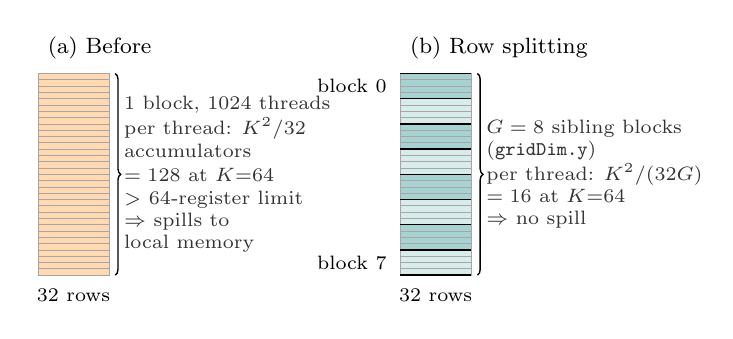
\begin{tikzpicture}[
    font=\footnotesize, x=1mm, y=1mm,
    row/.style={draw=black!35, line width=0.25pt},
    note/.style={font=\scriptsize, text=black!80, inner sep=0.8pt, align=left},
    brace/.style={decorate, decoration={brace, amplitude=2pt}, line width=0.5pt}]

% (a) defective: one block owns the whole 32-row tile row
\node[anchor=south west] at (0,27.4) {(a) Before};
\foreach \r in {0,...,31}
  \draw[row, fill=orange!30] (0,26-0.8*\r) rectangle (9,26.8-0.8*\r);
\draw[brace] (9.8,26.8) -- (9.8,1.2) node[midway, right=2.2pt, note]
  {1 block, 1024 threads\\[1pt]per thread: $K^2/32$\\accumulators\\[1pt]$= 128$ at $K{=}64$\\$>$ 64-register limit\\$\Rightarrow$ spills to\\local memory};

% (b) row splitting: G = 8 sibling blocks, 4 rows each
\node[anchor=south west] at (46,27.4) {(b) Row splitting};
\foreach \g in {0,...,7}
  \foreach \r in {0,...,3} {
    \pgfmathtruncatemacro{\shade}{mod(\g,2) == 0 ? 35 : 15}
    \draw[row, fill=teal!\shade] (46,26-3.2*\g-0.8*\r) rectangle (55,26.8-3.2*\g-0.8*\r);
  }
\foreach \g in {0,...,7}
  \draw[line width=0.5pt] (46,26.8-3.2*\g) -- (55,26.8-3.2*\g);
\draw[line width=0.5pt] (46,1.2) -- (55,1.2);
\node[font=\scriptsize, anchor=east] at (45.5,25.2) {block 0};
\node[font=\scriptsize, anchor=east] at (45.5,2.8) {block 7};
\draw[brace] (55.8,26.8) -- (55.8,1.2) node[midway, right=2.2pt, note]
  {$G = 8$ sibling blocks\\(\texttt{gridDim.y})\\[1pt]per thread: $K^2/(32G)$\\$= 16$ at $K{=}64$\\$\Rightarrow$ no spill};
\node[font=\scriptsize, anchor=north] at (4.5,0.7) {32 rows};
\node[font=\scriptsize, anchor=north] at (50.5,0.7) {32 rows};
\end{tikzpicture}

\caption{Row splitting in the scalar baseline kernel at $K=64$. (a) One 1024-thread block owned a whole 32-row tile row, so each thread held $K^2/32$ accumulators and spilled. (b) $G$ sibling blocks share the tile row, which cuts the per-thread set to $K^2/(32G)$ with the same arithmetic order.}
\label{fig:rowsplit}
\end{figure}

\begin{table}[!t]
\caption{Audit of the Scalar FP32 Baseline Before and After Row Splitting (Netflix, RTX 3060). Compute Speedup Is APR-BALS over the Baseline Excluding the RMSE Check}
\label{tab:baselineaudit}
\centering
\footnotesize
\renewcommand{\arraystretch}{1.1}
\setlength{\tabcolsep}{4pt}
\begin{tabular}{lcc}
\toprule
 & \textbf{Defective} & \textbf{Corrected} \\
\midrule
Rows per block & 32 & $32/G$ \\
Stack/thread, $K{=}48$ & 280 B & 0--64 B \\
Stack/thread, $K{=}64$ & 656 B & 0--64 B \\
Gram GFLOP/s, $K{=}48$ & 63 & 249--277 \\
Gram GFLOP/s, $K{=}64$ & 51 & 187--201 \\
Compute speedup, $K \ge 48$ & 30--44$\times$ & 12.8--17.2$\times$ \\
\bottomrule
\end{tabular}
\end{table}

Three checks bound the corrected baseline. First, \texttt{ptxas} reports no spill stores for any scalar template that the dispatch launches. Second, the kernel sustains 187--280~GFLOP/s, about $2\%$ of FP32 peak, with neither DRAM (42.2\%) nor SM (29.7\%) throughput saturated (Section~\ref{ssec:analysis}), which is consistent with a latency-bound workload involving irregular gathers and atomic flushes. Third, our faithful reimplementation of BALS (Section~\ref{ssec:balsequiv}) runs within $0.5\%$ of the baseline per sweep at 14 of 20 dataset--rank pairs and is never more than $1.21\times$ faster. The baseline is not the fastest FP32 design, however: cuMF\_als, which uses a different Gram kernel and a CG solver, is $1.4$--$4.4\times$ faster per sweep at $K \ge 32$. Ratios over the baseline therefore isolate the dispatch within one design, and the comparison with cuMF\_als (Section~\ref{ssec:cumfals}) is the conservative measure of the overall advantage.

\subsection{Blocked Batched Cholesky Solver}
\label{ssec:cholesky}

Each system $(A_u + \lambda n_u I)\mathbf{x}_u = \mathbf{b}_u$ is solved on the GPU. The regularization term is added to the diagonal inside the solver, so both precision paths solve identical systems. At $K=16$, one thread factorizes one system in registers, which beat a warp-cooperative design by about $1.3\times$. For $K \ge 32$, a first warp-cooperative packed solver reached only about $2\%$ of FP32 peak because each system required $2K$ block-wide barriers and $K$ serial dot-product chains. The production solver instead assigns one thread block per system and works on $16 \times 16$ shared-memory tiles with a padded row pitch of 17 that avoids bank conflicts. It combines four techniques (Fig.~\ref{fig:cholesky}):
(i)~\textit{blocked panels}: one warp factorizes each diagonal tile, all threads solve the panel below it, and the trailing update uses $2 \times 2$ register-blocked dot products, cutting block-wide barriers from $2K$ to about $3K/16$; (ii)~a \textit{folded forward solve}, which carries the right-hand side through the panels as an extra row; (iii)~an \textit{inverse-diagonal backward solve}, which stores each diagonal factor's inverse in the unused upper half of its tile, so back substitution becomes one matrix--vector product per tile column; and (iv)~\textit{overlapped factorization}, in which warp~0 factorizes the next diagonal tile while the other warps finish the trailing update, hiding the serial phase of every panel but the first.
A host-precomputed scatter map with 16-byte loads further speeds up the load phase, bit-identically. The resulting solver is $1.86\times$, $1.93\times$, $2.08\times$, and $2.26\times$ faster than the packed design at $K = 32$, 48, 64, and 96, and it uses 56 registers per thread (40 in the FP16-tile variant of Section~\ref{ssec:fp16solver}) with no spills at every $K$.

\begin{figure}[!t]
\centering
% Tiled blocked Cholesky solver, one-column width (3.5 in).
% Same type sizes as the other TikZ figures: 8 pt tiles and lanes, 7 pt labels.
\begin{tikzpicture}[
    font=\footnotesize,
    >={Stealth[length=3pt]},
    t/.style={draw=black!55, minimum size=6.4mm, inner sep=0pt, line width=0.4pt},
    potrf/.style={t, fill=orange!22},
    trsm/.style={t, fill=blue!12},
    upd/.style={t, fill=teal!14},
    idle/.style={t, fill=black!4},
    lane/.style={draw, rounded corners=1pt, minimum height=5.2mm, inner sep=1pt, line width=0.4pt, align=center},
    lbl/.style={font=\scriptsize\itshape, text=black!65, inner sep=1pt}]

% (a) tile view at panel k = 1 of a K = 64 system (4 x 4 tiles of 16 x 16)
\foreach \i in {0,...,3} {
  \foreach \j in {0,...,3} {
    \ifnum\j>\i
      \node[idle] at (0.64*\j, -0.64*\i) {};
    \else\ifnum\j=0
      \node[t, fill=black!15] at (0.64*\j, -0.64*\i) {};
    \else\ifnum\i=1
      \node[potrf] at (0.64*\j, -0.64*\i) {P};
    \else\ifnum\j=1
      \node[trsm] at (0.64*\j, -0.64*\i) {T};
    \else
      \node[upd] at (0.64*\j, -0.64*\i) {U};
    \fi\fi\fi\fi
  }
}
\foreach \i in {0,...,3} {
  \node[t, minimum width=3mm, fill=yellow!25] at (2.72, -0.64*\i) {};
}
\node[lbl, above=0.5mm] at (2.72, 0.32) {$\mathbf{b}_u$};
\node[lbl, above=0.5mm] at (0.96, 0.32) {(a) panel $k{=}1$, $K{=}64$};

% (b) phase overlap between warp 0 and the remaining warps
\begin{scope}[xshift=4.35cm, yshift=-0.2cm]
\node[lbl, anchor=south west] at (0, 0.2) {(b) overlap per panel};
\node[lbl, anchor=east] at (0, -0.35) {warp 0};
\node[lbl, anchor=east] at (0, -1.05) {others};
\node[lane, fill=orange!22, minimum width=15.5mm, anchor=west] at (0.05, -0.35) {P, tile $k{+}1$};
\node[lane, fill=blue!12, minimum width=9mm, anchor=west] at (1.70, -0.35) {T};
\node[lane, fill=teal!14, minimum width=25.5mm, anchor=west] at (0.05, -1.05) {U, panel $k$};
\draw[densely dashed, black!60] (2.70, 0.05) -- (2.70, -1.45);
\node[lbl, anchor=north] at (2.70, -1.45) {barrier};
\end{scope}

% key
\node[lbl, anchor=north west] at (-0.32, -2.25)
  {P: diagonal factor\quad T: triangular solve\quad U: trailing update\quad grey: completed panel};
\end{tikzpicture}

\caption{Tiled blocked Cholesky solver for $K \ge 32$. (a) Tile roles at panel $k{=}1$ of a $K{=}64$ system; the right-hand side $\mathbf{b}_u$ is carried through the panels. (b) Warp~0 factorizes the next diagonal tile while the other warps apply the trailing update of the current panel.}
\label{fig:cholesky}
\end{figure}

\subsection{Execution Pipeline}
\label{ssec:pipeline}

Gram buffers for half a million entities do not fit in device memory, so each half-sweep processes batches of 60{,}000 entities. Gram assembly runs on one CUDA stream, and each finished batch is solved on a second, higher-priority stream using double-buffered Gram storage (lines~\ref{alg:tr:wait}--\ref{alg:tr:solve} of Algorithm~\ref{alg:training}); CUDA events enforce the two true dependencies. On both paths, the harness's RMSE kernel predicts from FP32 factors and reduces in double precision.

\subsection{Convergence Protocol and Fair Comparison}
\label{ssec:protocol}

Both paths follow the same protocol. The factors start from the same seeded $U(0, 0.2)$ initialization, as in cuMF, and $\lambda = 0.048$ throughout. There is no separate validation split: $\lambda$ was selected on the test ratings (Section~\ref{ssec:weightedlambda}), whereas the thresholds and the momentum coefficient were chosen by wall time and stability. Absolute RMSE values may therefore be slightly optimistic; both paths share $\lambda$, so their comparison is unaffected. The train RMSE is evaluated every five sweeps, and training stops when it changes by less than $10^{-3}$ between two checks, with a limit of 50 sweeps. The check interval is thus part of the rule and is fixed.

The baseline is the same binary with a zeroed density array, which routes every entity to the scalar tier and suppresses the WMMA launches. Storage format, batching, solver, RMSE kernel, convergence rule, and stream pipeline are therefore shared. Tile structures are built from training data only, regularization enters only through the solver diagonal, and convergence is judged only on training error. Two restrictions are deliberate. The scalar kernel computes the full $K \times K$ Gram matrix, because a triangular variant ran slower; weakening the baseline was not acceptable. Only $K \in \{16, 32, 48, 64, 96\}$ is supported, because the WMMA shape requires multiples of 16 and each value needs its own register-tile instantiation. Zeroing the density array also disables the FP16 staging inside the scalar kernel, so the two-path ratio covers that optimization as well; Section~\ref{ssec:precisioniso} separates the effects with a single-kernel ablation.
